\documentclass[border=5mm]{standalone}
\usepackage{tikz}
\usetikzlibrary{shapes.geometric, arrows.meta}

\begin{document}

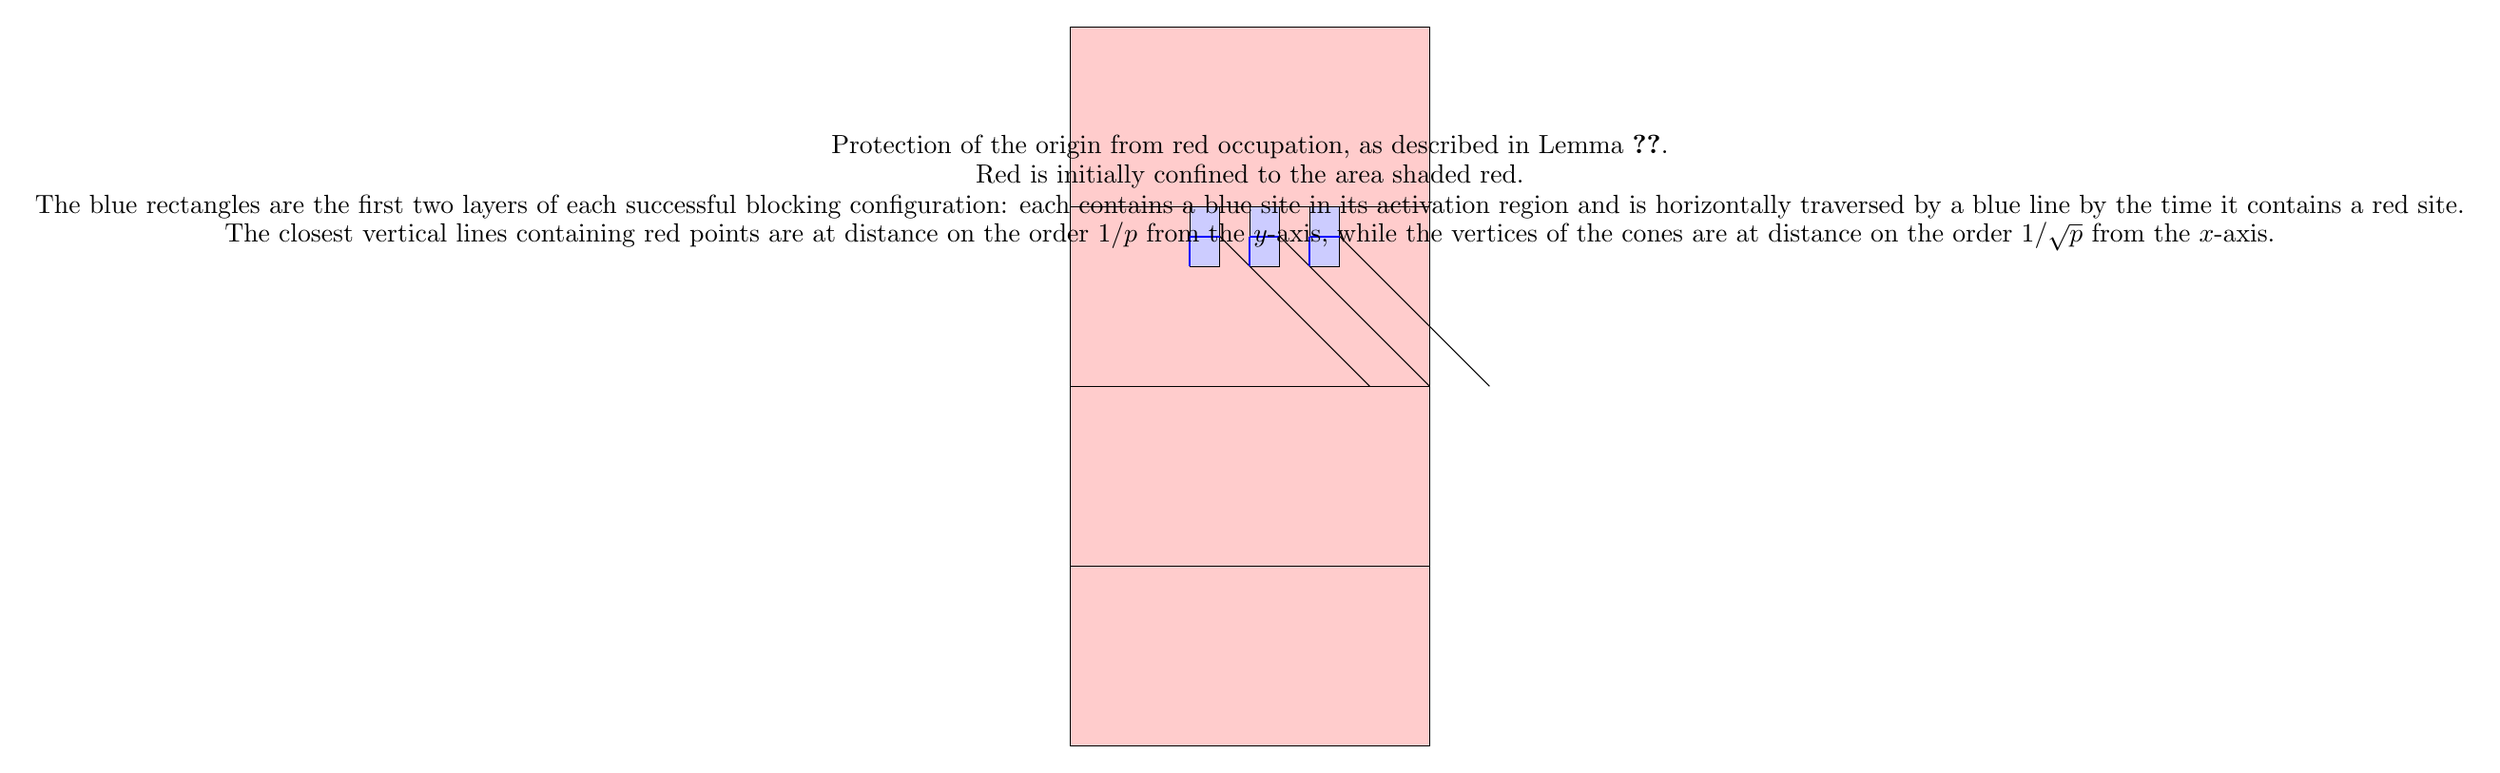
\begin{tikzpicture}[scale=0.8]
    % Define colors
    \definecolor{lightpink}{RGB}{255, 204, 204}
    \definecolor{darkpink}{RGB}{255, 102, 102}
    
    % Draw the grid and shading
    \draw[fill=lightpink] (-3, -3) rectangle (3, 3);
    \draw[fill=lightpink] (-3, 3) -- (-3, 6) -- (3, 6) -- (3, 3) -- cycle;
    \draw[fill=lightpink] (-3, -3) -- (-3, -6) -- (3, -6) -- (3, -3) -- cycle;
    \draw[fill=lightpink] (-3, 0) rectangle (3, 3);
    
    % Draw the cones
    \foreach \i in {-1, 0, 1} {
        \draw[fill=darkpink] (\i, 3) -- (\i+1, 2) -- (\i+2, 1) -- (\i+3, 0) -- cycle;
    }
    
    % Draw the blue rectangles
    \foreach \i in {-1, 0, 1} {
        \draw[fill=blue!20] (\i, 2) rectangle (\i+0.5, 3);
    }
    
    % Draw the blue horizontal lines
    \foreach \i in {-1, 0, 1} {
        \draw[blue, thick] (\i, 2.5) -- (\i+0.5, 2.5);
    }
    
    % Draw the blue vertical lines
    \foreach \i in {-1, 0, 1} {
        \draw[blue, thick] (\i, 2) -- (\i, 2.5);
    }
    
    % Add the text
    \node at (0, 4) {Protection of the origin from red occupation, as described in Lemma~\ref{protection lemma}.};
    \node at (0, 3.5) {Red is initially confined to the area shaded red.};
    \node at (0, 3) {The blue rectangles are the first two layers of each successful blocking configuration: each contains a blue site in its activation region and is horizontally traversed by a blue line by the time it contains a red site.};
    \node at (0, 2.5) {The closest vertical lines containing red points are at distance on the order $1/p$ from the $y$-axis, while the vertices of the cones are at distance on the order $1/\sqrt{p}$ from the $x$-axis.};
\end{tikzpicture}

\end{document}